 \let\negmedspace\undefined
\let\negthickspace\undefined
\documentclass[journal]{IEEEtran}
\usepackage[a5paper, margin=10mm, onecolumn]{geometry}
%\usepackage{lmodern} % Ensure lmodern is loaded for pdflatex
\usepackage{tfrupee} % Include tfrupee package

\setlength{\headheight}{1cm} % Set the height of the header box
\setlength{\headsep}{0mm}     % Set the distance between the header box and the top of the text
\usepackage{gvv-book}
\usepackage{gvv}
\usepackage{cite}
\usepackage{amsmath,amssymb,amsfonts,amsthm}
\usepackage{algorithmic}
\usepackage{graphicx}
\usepackage{textcomp}
\usepackage{xcolor}
\usepackage{txfonts}
\usepackage{listings}
\usepackage{enumitem}
\usepackage{mathtools}
\usepackage{gensymb}
\usepackage{comment}
\usepackage[breaklinks=true]{hyperref}
\usepackage{tkz-euclide} 
\usepackage{listings}
% \usepackage{gvv}                                        
\def\inputGnumericTable{}                                 
\usepackage[latin1]{inputenc}                                
\usepackage{color}                                            
\usepackage{array}                                            
\usepackage{longtable}                                       
\usepackage{calc}                                             
\usepackage{multirow}                                         
\usepackage{hhline}                                           
\usepackage{ifthen}                                           
\usepackage{lscape}



\usepackage{amsmath,amssymb}
\usepackage{booktabs}
\usepackage{tikz}
\usetikzlibrary{arrows.meta,angles,quotes}





\begin{document}

\bibliographystyle{IEEEtran}
\vspace{3cm}

\title{4.8.19}
\author{AI25BTECH11023 - Pratik R}
% \maketitle
% \newpage
% \bigskip
{\let\newpage\relax\maketitle}

\renewcommand{\thefigure}{\theenumi}
\renewcommand{\thetable}{\theenumi}
\setlength{\intextsep}{10pt} % Space between text and floats


\numberwithin{equation}{enumi}
\numberwithin{figure}{enumi}
\renewcommand{\thetable}{\theenumi}


\section*{\textbf{Question}}
If the distance of the point $(1,1,1)$ from the plane $x-y+z+ \lambda = 0$ is$\frac{5}{\sqrt{3}}$, find the value(s) of $\lambda$.

\subsection*{\textbf{Solution:}} 
Equation of plane is given by
\begin{align}
	\vec{n}^\top \vec{x} = -\lambda;
\end{align}
where $\vec{n}^\top = \myvec{1&-1&1}$. \\

Let the distance of point \vec{P}(1,1,1) from the plane is d.
\begin{align}
	d = \dfrac{||\vec{n}^\top \vec{P} + \lambda||}{||\vec{n}||}
\end{align}
then value of $\lambda $ is given by

\begin{align}
	\lambda = + d||\vec{n}||-\vec{n}^\top \vec{P} \text{ or} \\
	\lambda = - d||\vec{n}||-\vec{n}^\top \vec{P}
\end{align}
Solving these Equations we get
\begin{align}
   \implies \lambda &= +4 \\
    &=-6
\end{align}
\newpage

\begin{figure}[H]
\centering
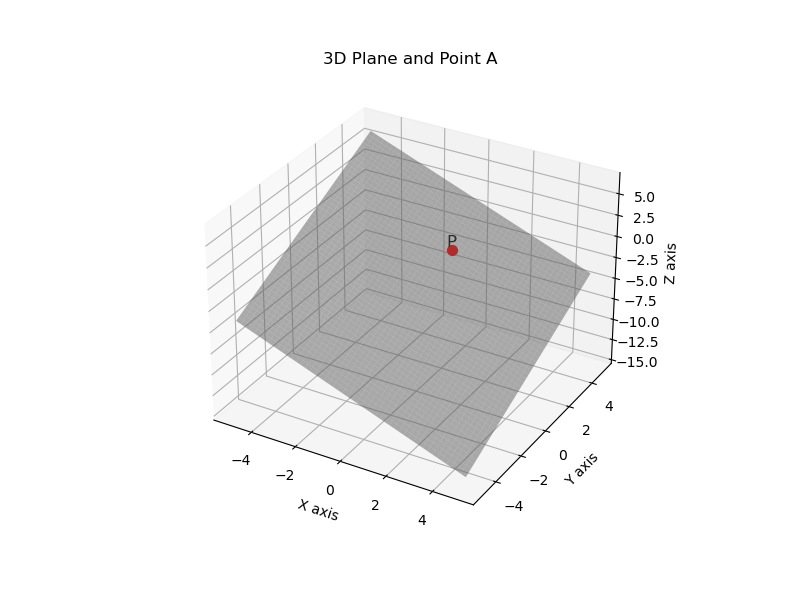
\includegraphics[width=0.7\columnwidth]{figs/fig1.png} 
\caption{plane}
\label{}
\end{figure}
\begin{figure}[H]
\centering
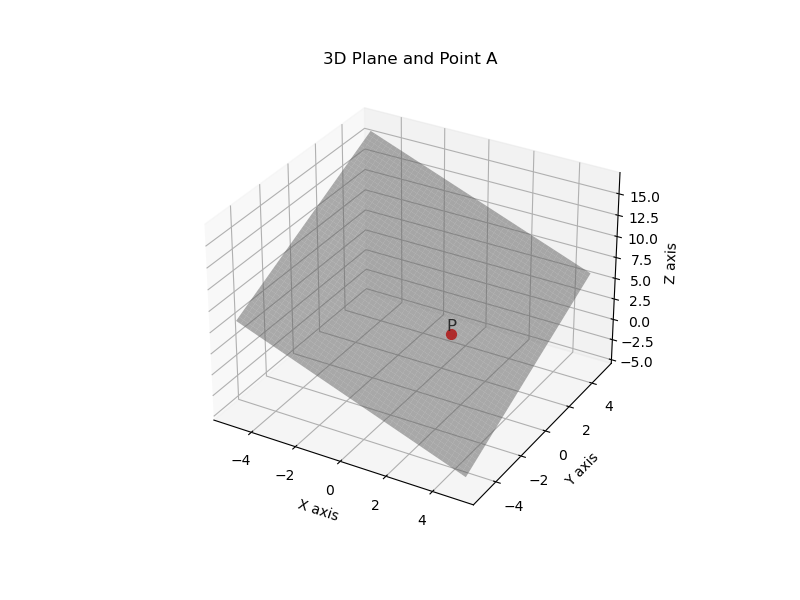
\includegraphics[width=0.7\columnwidth]{figs/fig2.png} 
\caption{plane}
\label{}
\end{figure}
\end{document}
